\begin{figure}
  \centering
  \begin{tikzpicture}
    \node[inner sep=0pt] (img1) at (0,0.28\textwidth)
         {
\includegraphics[width=0.45\textwidth]{./img/raw/vp-visibiliteit/wf.png}};
    \node[inner sep=0pt] (img2) at (-0.2\textwidth,0)
         {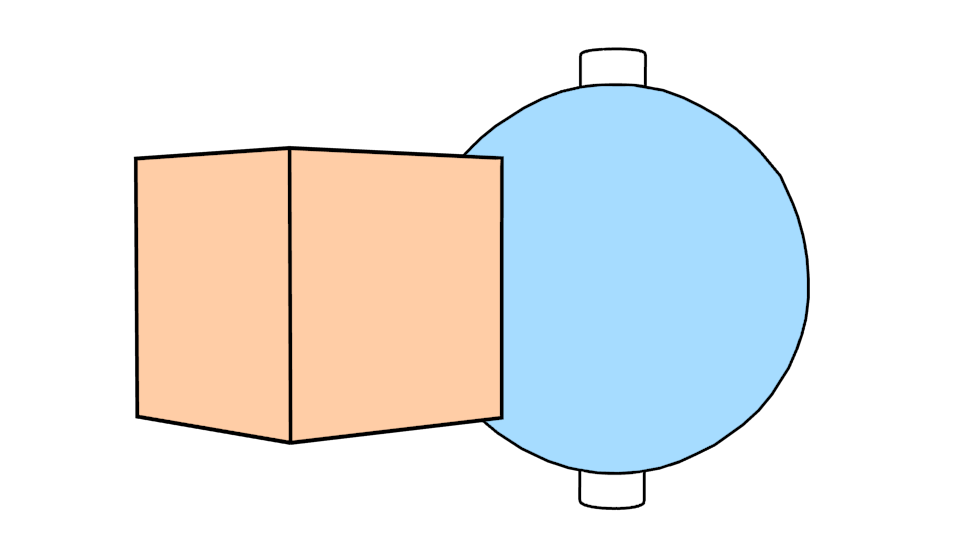
\includegraphics[width=0.45\textwidth]{./img/raw/vp-visibiliteit/cube.png}};
    \node[inner sep=0pt] (img3) at (0.2\textwidth,0)
         {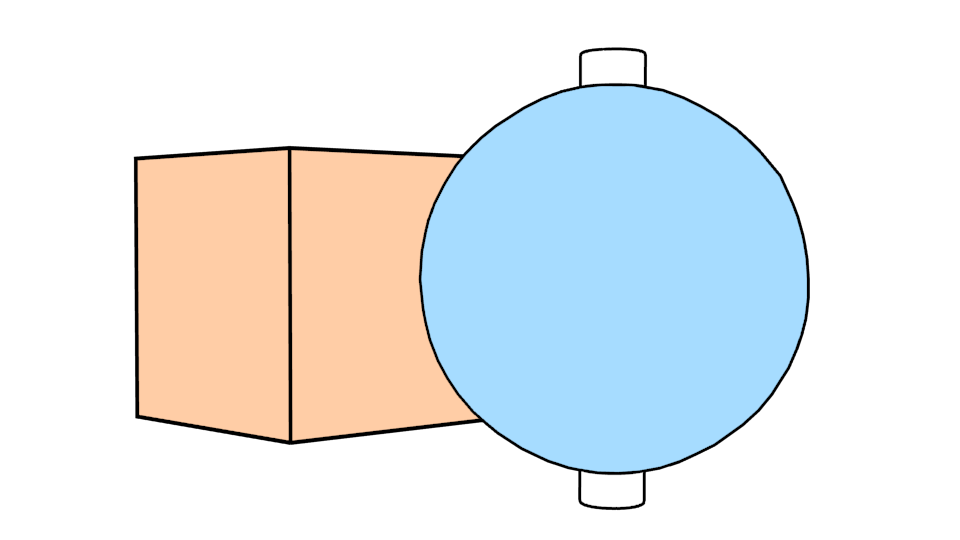
\includegraphics[width=0.45\textwidth]{./img/raw/vp-visibiliteit/sphere.png}};

    \draw[-latex] (img1) -- (img2) ;
    \draw[-latex] (img1) -- (img3) ;
  \end{tikzpicture}
  \caption{Visibiliteitsprobleem in een scene met meerdere primitieven.}
  \label{fig:vp-visibiliteit}
\end{figure}
